\section{Evaluation}
\label{sec:evaluation}
\begin{figure*}[t]
        \centering
        \begin{subfigure}[b]{0.3\textwidth}
                \centering
                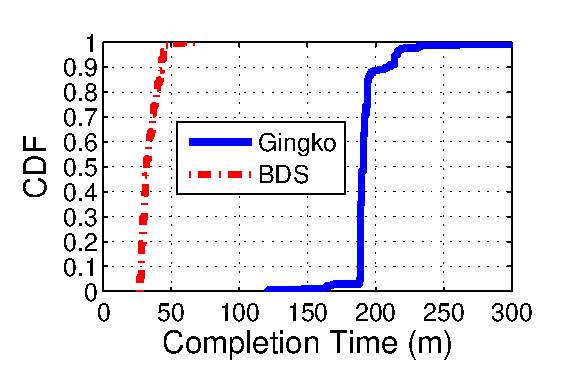
\includegraphics[width=\textwidth]{images/BDSvsAnon_overall_v2.eps}
                \caption{Distribution of completion time.}
                \label{fig:BDSvsAnon:overall}
        \end{subfigure}
        \begin{subfigure}[b]{0.3\textwidth}%@X:\6 PieBridge\simulation\beijing\3 Applications\plot
                \centering
                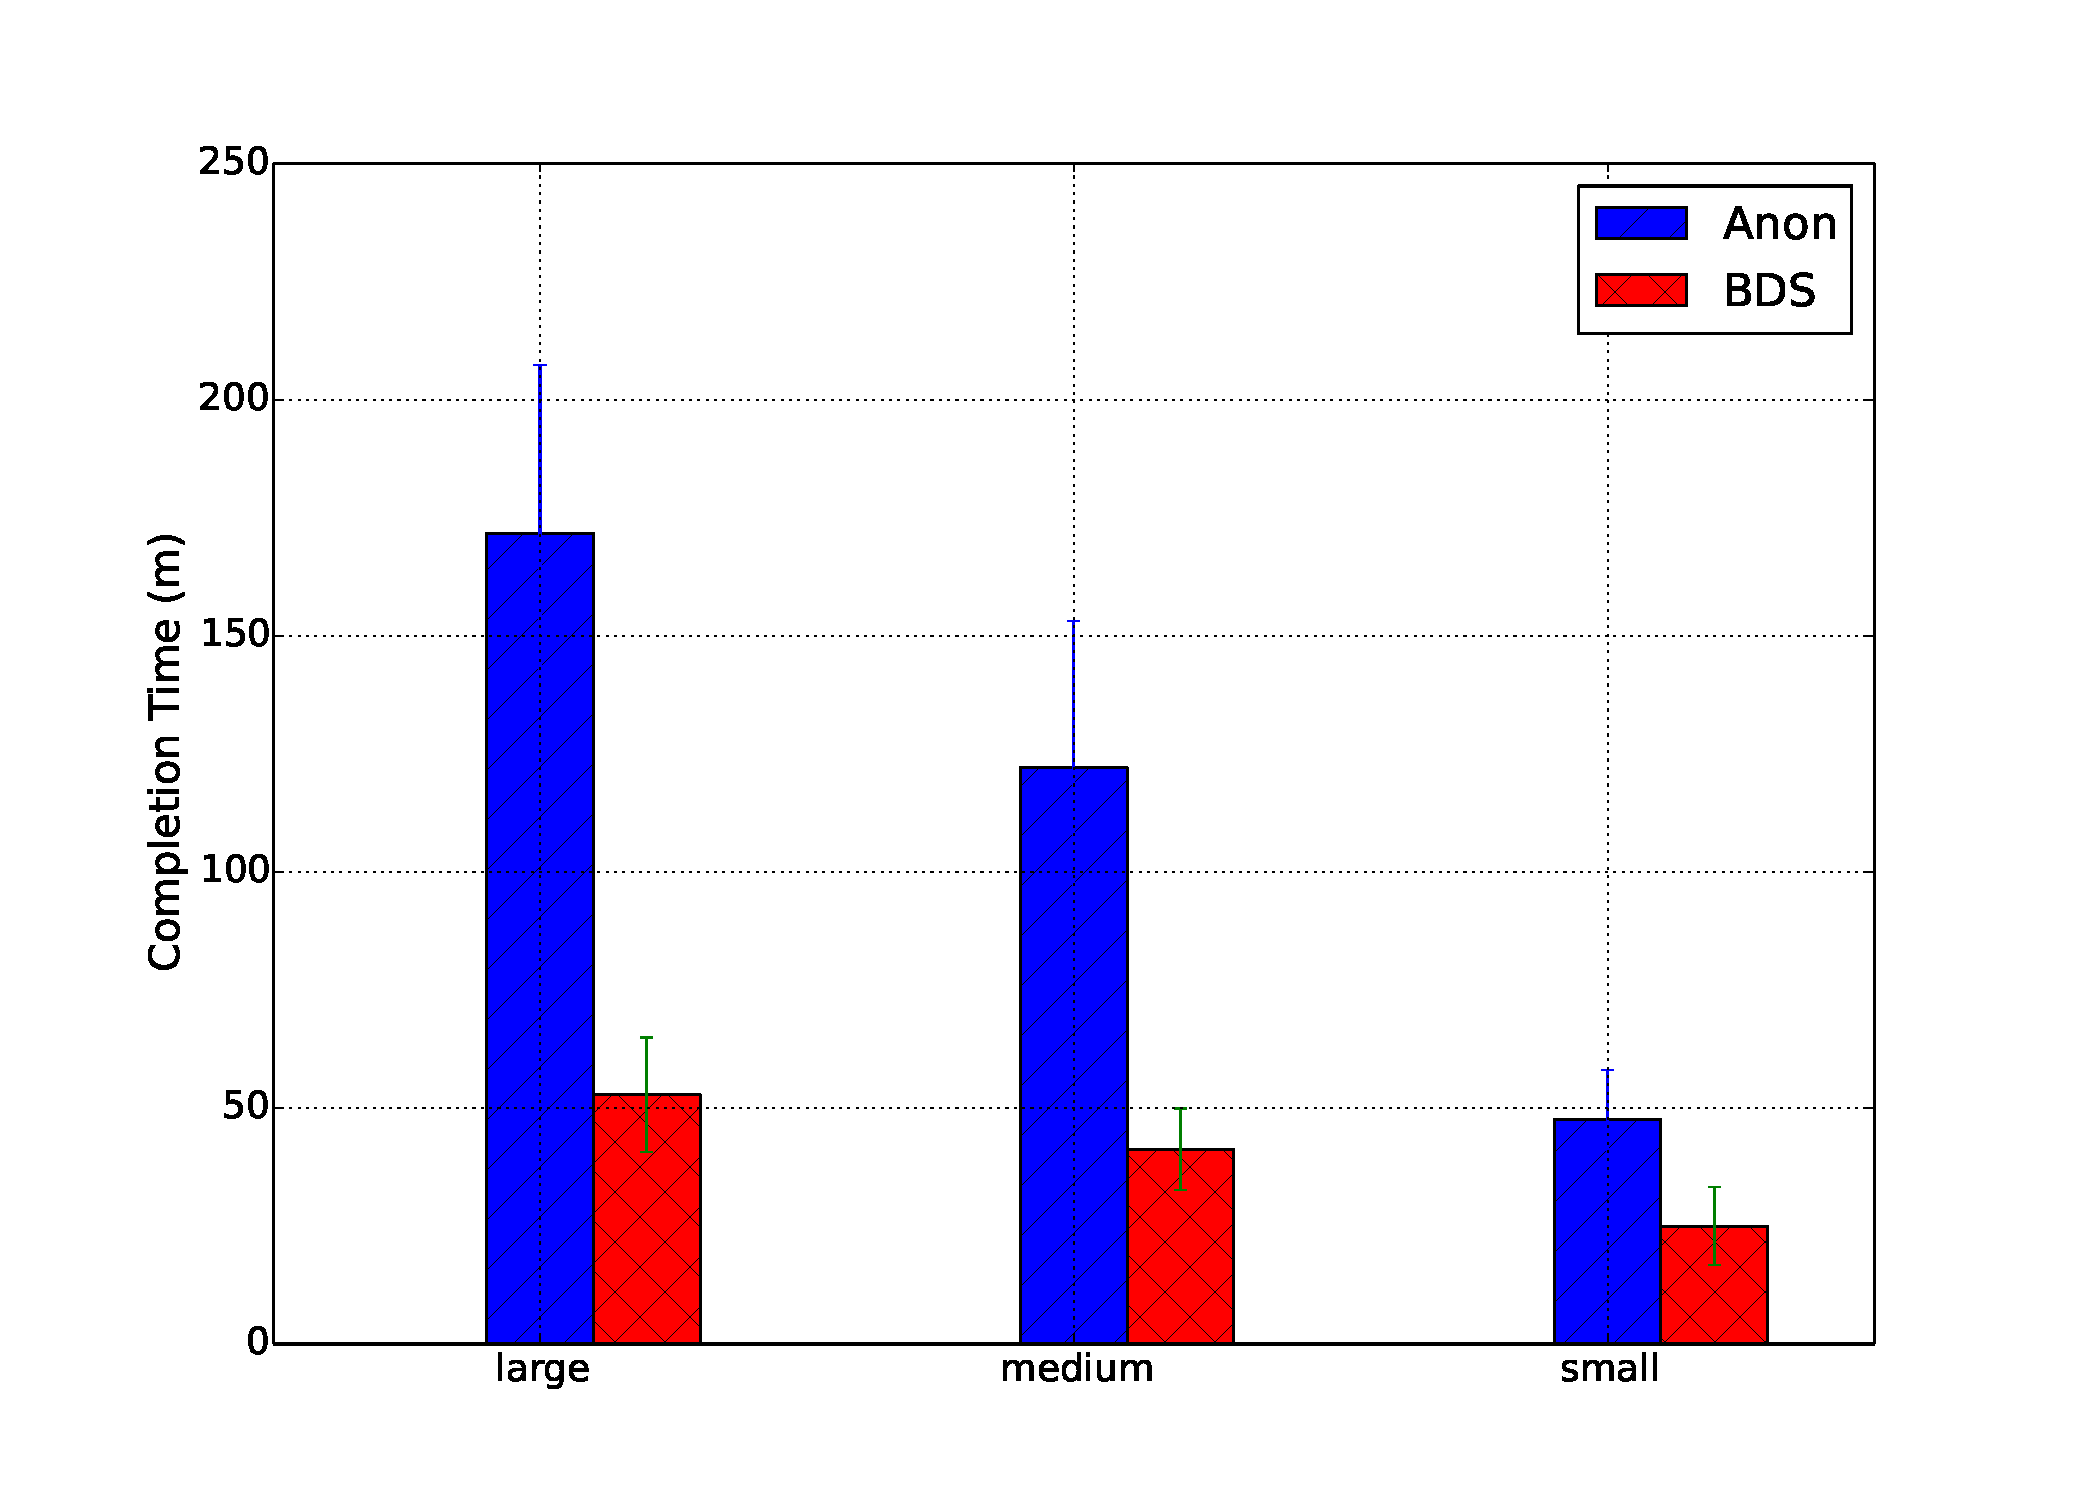
\includegraphics[width=\textwidth]{images/BDS_VS_ANON_v2.eps}
                \caption{Comparison by application types.}
                \label{fig:BDSvsAnon:FCT}
        \end{subfigure}
        \begin{subfigure}[b]{0.3\textwidth}
                \centering
                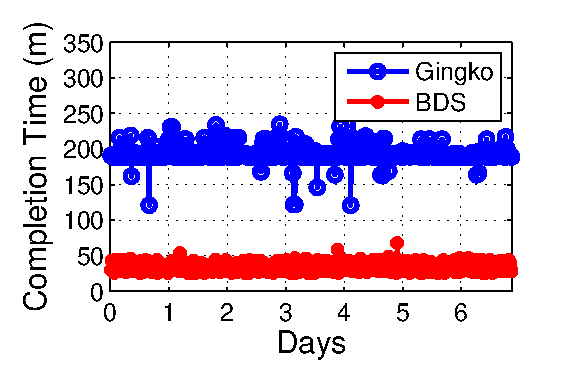
\includegraphics[width=\textwidth]{images/BDSvsAnon_time_v2.eps}
                \caption{Comparison by completion time.}
                \label{fig:BDSvsAnon:time}
        \end{subfigure}
        \tightcaption{[\name vs. \alg (\company's existing solution)] Results from pilot deployments.}
        \label{fig:BDSvsAnon}
\vspace{-0.4cm}
\end{figure*}

%To evaluate \name, we integrated our end-to-end prototype in
%\company, and ran a pilot deployment of \name.
Using a combination of pilot deployment in \company's DCs,
trace-driven simulation, and microbenchmarking, we show that:
\begin{packedenumerate}
\item \name completes inter-DC multicast 3-5$\times$ faster than
\company's existing solutions, as well as other baselines used in
industry (\Section\ref{subsec:evaluation:centralized}).

%\NEW{ DELETE:
%\item \name significantly reduces the incidents of interferences
%between bulk-data multicast traffic and latency-sensitive traffic
%(\Section\ref{subsec:evaluation:separation}).
%}

\item \name can scale to the traffic demand of a large online
service provider, tolerate various failure scenarios, and achieves
close to optimal flow completion time
(\Section\ref{subsec:evaluation:benchmarks}).


\NEW{
\item \newname can: 1. further complete inter-DC multicast 1.2 to 1.3 times faster than \name, 2. predict the bandwidth utilization of online traffic with about 95\% accuracy, 3. increase bandwidth utilization when online traffic is in valley, while reduces the bulk data transfer when online traffic bursts, 4. achieve near real-time scheduling with quite low computation overhead
(\Section\ref{subsec:evaluation:improvements}).
}
\end{packedenumerate}

\subsection{Performance improvement over existing solutions}
\label{subsec:evaluation:centralized}

\subsubsection{Methodology}
\

\mypara{Baselines}
We compare \name with three existing solutions: \alg (\company's
existing decentralized inter-DC multi-cast strategy),
Bullet~\cite{kostic2003bullet}, and Akamai's overlay
network~\cite{Andreev2013Designing} (a centralized strategy for
multicasting live videos).


\mypara{Pilot deployment}
We choose several services with different data sizes, and run
A/B testing in which we run \name instead of \company's default
solution \alg for the same hours in several randomly chosen days.

\mypara{Trace-driven simulation}
Complementary to the pilot deployment on real traffic, we also use
trace-driven simulation to evaluate \name on a larger scale.
We simulate the other two overlay multicast techniques using the
same topology, number of servers, and link capacities as \name, and
replay inter-DC multicast data requests in the same chronological
order as in the pilot deployment.

\subsubsection{\name vs. \alg}
\label{subsubsec:name-vs-alg}
\

We begin by evaluating \name and \alg on one service that needs to
distribute 70~TB data from one source DC to ten destination DCs.
Figure~\ref{fig:BDSvsAnon:overall} shows the cumulative distribution
function (CDF) of the completion time on each destination server. We can
see that the median completion time of \name is 35 minutes,
$5\times$ faster than \alg, where most DCs takes 190 minutes to
get the data.

To generalize the finding, we pick three applications whose data
volumes are large, medium and small, and compare \name's and \alg's
mean (and standard deviation) of completion time for each application
in Figure~\ref{fig:BDSvsAnon:FCT}.
We see that \name consistently outperforms \alg, and has less
performance variance. We also see that \name has greater improvement
in applications with larger data sizes. Finally,
Figure~\ref{fig:BDSvsAnon:time} shows the timeseries of the mean
completion time of \name and \alg in one randomly chosen application,
and we see that \name consistently outperforms \alg by 4$\times$.

\subsubsection{\name vs. other overlay multicast techniques}
\

Table~\ref{table:versusAkamai} compares \name with two other
baselines, Bullet and Akamai's overlay network, using trace-driven
simulation. We show the results in three setups. In the baseline evaluations,
we send 1TB data from one DC to 11 DCs, each has 100 servers, and
the upload and download link capacities are set to be 20MBs. In the
large-scale evaluations, we send 10TB data between the same DCs, each with
1000 servers. In the rate-limited evaluations, the setup is the same as that in the baseline experiments
except the server upload and download rate limit set to be 5MBs.
We see that \name achieves 3$\times$ shorter completion time than
Bullet and Akamai in the baseline setup, and over 4$\times$ shorter
completion time in the large-scale and small bandwidth setups, which
corroborates the findings in \Section\ref{subsubsec:name-vs-alg} that
\name has greater improvement when data sizes are large.

\begin{table}[t]
\begin{center}
\resizebox{3in}{!}{
%\begin{tabular}{p{2cm}<{\centering}|p{2cm}<{\centering}}
\begin{tabular}{| c | c| c| c|}
\hline
 \rowcolor[gray]{0.9}
\textbf{Solution} & \textbf{Baseline} & \textbf{Large Scale} & \textbf{Rate Limit} \\
\hline \hline
Bullet & $28m$ & $82m$ & $171m$\\
\hline
Akamai & $25m$ & $87m$ & $138m$\\
\hline
\name & $9.41m$ & $20.33m$ & $38.25m$\\
\hline
\end{tabular}
}
\end{center}
\caption{[\name vs. Bullet \cite{kostic2003bullet}, Akamai \cite{Andreev2013Designing}] Completion time of the three solutions in  trace-driven simulation.}
%\caption{Average completion time of Bullet \cite{kostic2003bullet}, Akamai \cite{Andreev2013Designing} and \name.}
\label{table:versusAkamai}
%\vspace{-0.4cm}
\end{table}

%\subsection{Benefits of coordinated bandwidth allocation}
%\label{subsec:evaluation:separation}
%\begin{figure}[t]
%  \centering
%  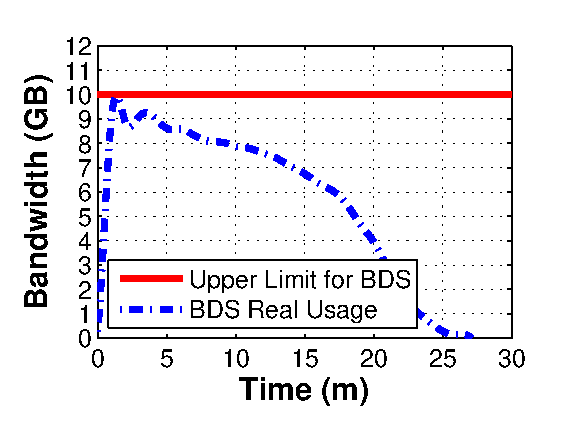
\includegraphics[width=45mm]{images/Quota_v2.eps}%DrawLink.m
%  \tightcaption{\color{red}{DELETE: The effectiveness of bandwidth separation.}}
%  \label{fig:quota}
%\vspace{-0.4cm}
%\end{figure}
%
%To reduce the incidences of negative interference between bulk-data
%multicast traffic and latency-sensitive traffic, \company sets a
%bandwidth limit of bulk data transfers on each link by the difference
%between the link capacity and the historical peak bandwidth of
%latency-sensitive traffic. Naturally, we can minimize the conflicts,
%if \name can keep the bulk-data multicast traffic within the bandwidth
%limit. To test \name's effectiveness at maintaining differentiation between
%bulk-data multicast traffic and latency-sensitive traffic, we set an
%10GB/s bandwidth limit to bulk data transfers.
%Figure~\ref{fig:quota} shows the actual bandwidth usage of \name on
%one inter-DC link. We can see that in \name the actual bandwidth used
%by bulk data is always below 10~GB/s.

%\begin{table}[t]
%\begin{center}
%\resizebox{3in}{!}{%
%%\begin{tabular}{p{2cm}<{\centering}|p{2cm}<{\centering}}
%\begin{tabular}{| c | c | c | c | c |}
%\hline
% \rowcolor[gray]{0.9}
%\textbf{System} & \textbf{Source DC egress link} & \textbf{$l_1$} & \textbf{$l_2$} & \textbf{$l_3$}\\
%\hline \hline
%\alg & 69.82\% & 53.09\% & 57.98\% & 63.01\% \\
%\hline
%\name & 70.55\% & 62.46\% & 63.23\% & 64.24\% \\
%\hline
%\end{tabular}
%}
%\end{center}
%\tightcaption{Average link utilizations of the source DC egress link and 3 inter-DC links ($l_1$, $l_2$, $l_3$) under \alg and \name.}
%\label{table:usage}
%\vspace{-0.4cm}
%\end{table}

\begin{figure*}[t]
        \centering
        \begin{subfigure}[b]{0.3\textwidth}
                \centering
                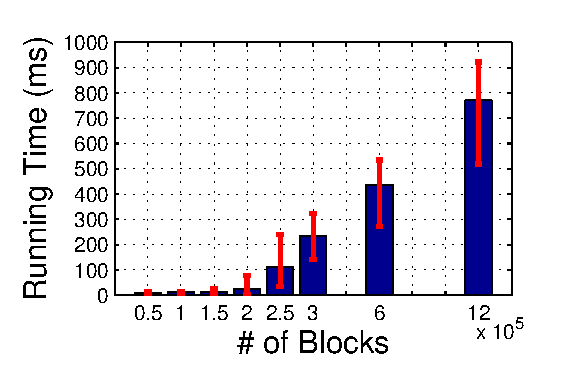
\includegraphics[width=50mm]{images/CPUvsBlk_v3.eps}% cpu.m replaced by running_time.m
                \caption{The controller running time.}
                \label{fig:scale:cpu}
        \end{subfigure}
        \begin{subfigure}[b]{0.3\textwidth}
                \centering
                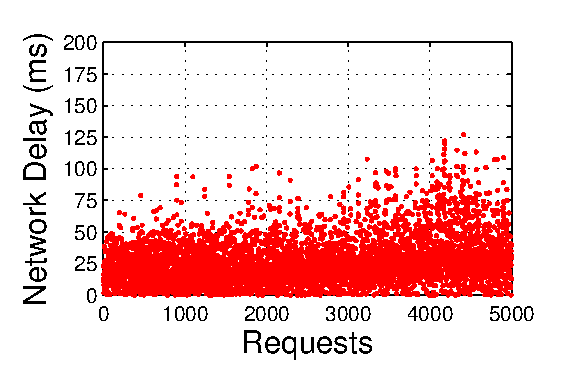
\includegraphics[width=50mm]{images/NetworkDelay.eps}%CDFofNetworkDelay -> Communication.m
                \caption{The inter-DC network delay.}
                \label{fig:scale:network}
        \end{subfigure}
        \begin{subfigure}[b]{0.3\textwidth}
                \centering
                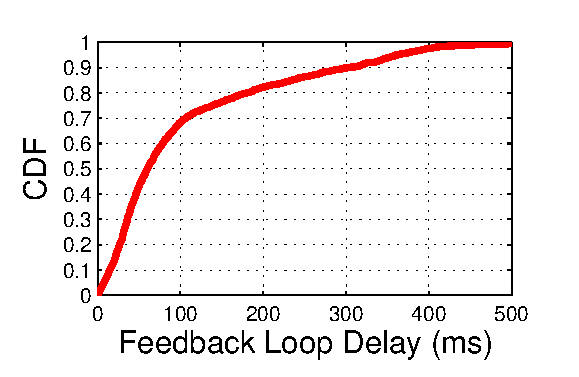
\includegraphics[width=50mm]{images/CDFofFeedbackLoopDelay.eps}
                \caption{Feedback loop delay.}
                \label{fig:scale:feedback}
        \end{subfigure}
        \tightcaption{[System scalability] Measurements on (a) controller running time, (b) network delay, (c) Feedback loop delay.}
        \label{fig:scale}
%\vspace{-0.4cm}
\end{figure*}

\begin{figure*}[t]
        \centering
        \begin{subfigure}[b]{0.3\textwidth}
                \centering
                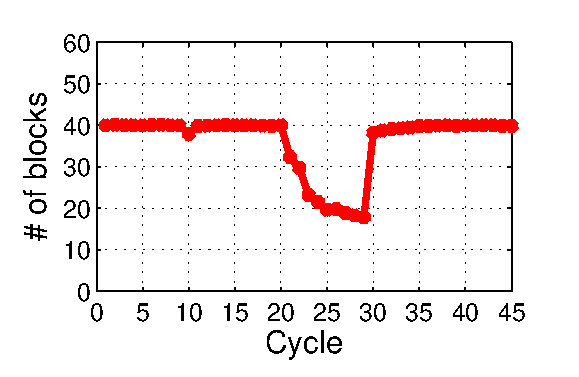
\includegraphics[width=50mm]{images/failure_v2.eps}%fail.m
                \caption{Average number of downloaded blocks per cycle under failures.}
                \label{fig:analysis:failure}
        \end{subfigure}
        \begin{subfigure}[b]{0.3\textwidth}
                \centering
                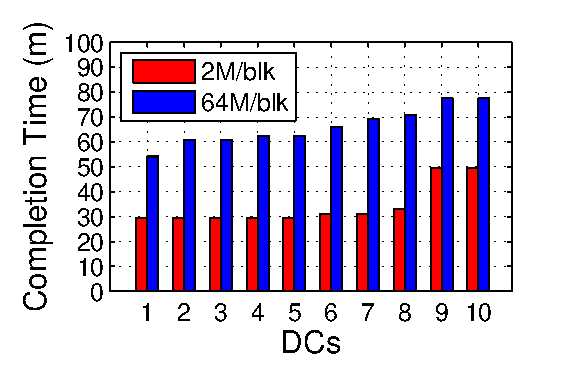
\includegraphics[width=50mm]{images/blkSize_v2.eps} %plotTCT_IDC.m
                \caption{Completion time under different block sizes.}
                \label{fig:analysis:blksize}
        \end{subfigure}
        \begin{subfigure}[b]{0.3\textwidth}
                \centering
                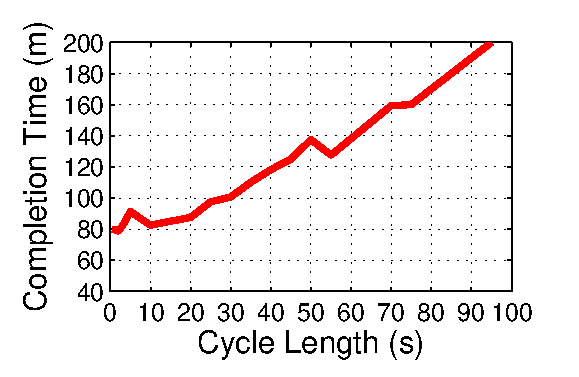
\includegraphics[width=50mm]{images/cycleDiff.eps}%cycleDiff.m
                \caption{Completion time under different cycle lengths.}
                \label{fig:analysis:cycleDiff}
        \end{subfigure}
%        \begin{subfigure}[b]{0.3\textwidth}
%                \centering
%                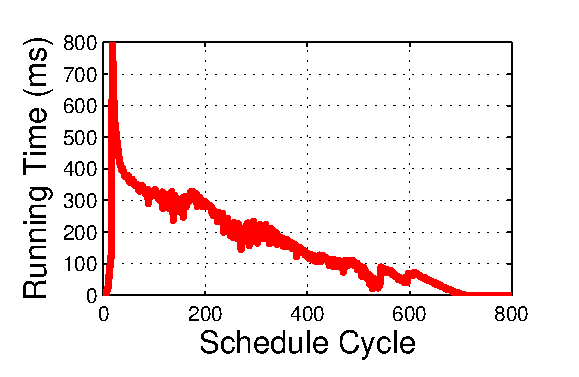
\includegraphics[width=50mm]{images/cycle.eps} %calculation_origin
%                \caption{Reduction on algorithm running time due to approximation.}
%                \label{fig:analysis:time}
%        \end{subfigure}
%        \begin{subfigure}[b]{0.3\textwidth}
%                \centering
%                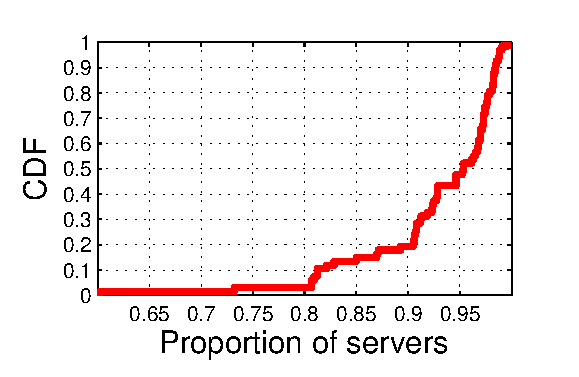
\includegraphics[width=50mm]{images/overlay.eps}
%                \caption{The proportion of blocks downloaded from the original source.}
%                \label{fig:analysis:overlay}
%        \end{subfigure}
        \tightcaption{\name's (a) fault tolerance, (b) sensitivity to different block sizes, and (c) different cycle lengths.}
        \label{fig:analysis}
%\vspace{-0.4cm}
\end{figure*}


%\jc{i'm totally lost... what's the point of this para?}
%As \name implements strict bandwidth separation between latency-sensitive traffic and bulk data transfers while still showing shorter completion time, does it occupy too much bandwidth on inter-DC links? To answer this question, we record the average utilizations of the egress link of the source DC and 3 randomly selected inter-DC links, denoted as $l_1,l_2$ and $l_3$. The result in Table \ref{table:usage} shows that link utilizations do not change much with \name. This is because \name spreads data transfers over bottleneck-disjoint paths, so it avoids transferring the same data on the same link.

%\begin{itemize}
%\item Draw a graph (what graph can you get on this?) to show with bandwidth separation, \name can reduce the incidents of delay on latency-sensitive traffic caused by bulk data transfers.%DrawLink.m
%\item Draw a graph (what graph can you get on this?) to show the link utilization does not change much with \name or with \company.%DrawUsage.m
%\end{itemize}

\subsection{Micro-benchmarks}
\label{subsec:evaluation:benchmarks}

Next, we use micro-benchmarking to evaluate \name along three metrics:
(1) scalability of the centralized control;
(2) fault tolerance; and
(3) optimality of \name parameters.

\subsubsection{Scalability}
\label{subsec:evaluation:benchmarks:scalability}
\

\mypara{Controller running time}
As the controller needs to decide the scheduling and routing of each
data block, the running time of the control logic naturally scales
with the number of blocks. Figure~\ref{fig:scale:cpu} shows the
running time as a function of the total number of blocks. We can see
that the centralized \name controller can update the scheduling and
routing decision within 800ms with $10^6$ blocks. To put this number
into perspective, in \company's DCs, the maximum number of simultaneous
outstanding data blocks is around $3\times 10^5$, for which \name can
finish updating the decisions within 300ms.

\mypara{Network delay} \name works in inter-DC networks, so the network delay among DCs is a key factor in the algorithm updating process. We recorded the network delay of 5000 requests and present the CDF in Figure \ref{fig:scale:network}. We can see that 90\% of the network delays are below $50ms$ and the average value is about $25ms$, which is less than 1\% of the decision updating cycle (3 seconds).

\mypara{Feedback loop delay} For centralized algorithms, a small feedback loop delay is essential for algorithmic scalability. In \name, this feedback loop consists of several procedures: status updating from agents to the controller, running of the centralized algorithm, and decision updating from the controller back to agents. We measure the delay of the whole process, as shown in the CDF of Figure \ref{fig:scale:feedback}, and find that in most cases (over 80\%), the feedback loop delay is lower than $200ms$. So we claim that \name demonstrates a short enough latency and is able to scale to even larger systems.

\begin{figure*}[t]
        \centering
        \begin{subfigure}[b]{0.3\textwidth}
                \centering
                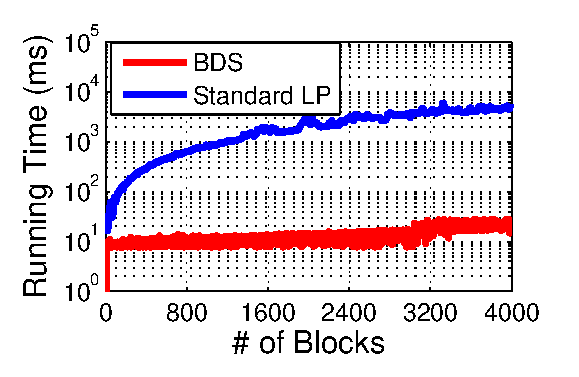
\includegraphics[width=50mm]{images/BDSvsLP_v2.eps} % BDSvsLP.m
                \caption{The reduction on algorithm running time of \name over standard LP.}
                \label{fig:further:BDSvsLP}
        \end{subfigure}
        \begin{subfigure}[b]{0.3\textwidth}
                \centering
                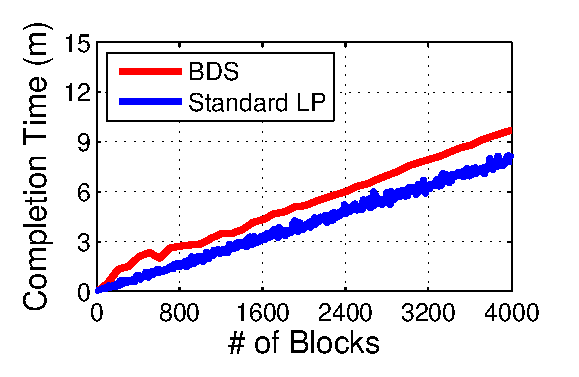
\includegraphics[width=50mm]{images/BDSvsLP_CT.eps}%BDSvsLP_CT -> Communication.m
                \caption{The near-optimality of \name to standard LP in small scale.}
                \label{fig:further:BDSvsLP_CT}
        \end{subfigure}
        \begin{subfigure}[b]{0.3\textwidth}
                \centering
                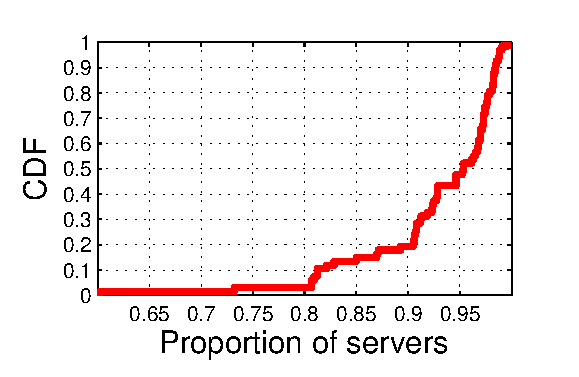
\includegraphics[width=50mm]{images/overlay.eps}
                \caption{The proportion of blocks downloaded from the original source.}
                \label{fig:further:overlay}
        \end{subfigure}
        \tightcaption{[In-depth analysis] on (a) reduction on algorithm running time, (b) near-optimality, and (c) effects of overlay transmission.}
        \label{fig:further}
%\vspace{-0.4cm}
\end{figure*}

%\tightsubsubsection{Algorithm adaptability.}\label{subsubsec:evaluation:adaptability}
\subsubsection{Fault tolerance}
\

%\mypara{Fault tolerance}
Here we examine the impact of the following failure scenario on the number of downloaded blocks per cycle. During cycles 0 to 9, \name works as usual, and one agent fails in the 10th cycle. The controller fails in the 20th cycle and recovers in the 30th cycle. Figure \ref{fig:analysis:failure} shows the average number of downloaded blocks per cycle. We find that the slight impact of agent failure only lasts for one cycle, and the system recovers in the 11th cycle. When the controller is unavailable, \name falls back to a default decentralized overlay protocol, resulting in graceful performance degradation. With the recovery of the controller, the performance recovers in the 30th cycle.

\subsubsection{Choosing the values of key parameters}\label{subsec:evaluation:benchmarks:parameters}
\

\mypara{Block size} In \name, the bulk data file is split into blocks and can be transferred on bottleneck-disjoint paths. But this introduces a tradeoff between scheduling efficiency and calculation overhead. We therefore conduct two series of experiments using different block sizes (2MB and 64MB). Figure \ref{fig:analysis:blksize} shows that the completion time in the 2MB/block scenario is 1.5 to 2 times shorter than that in the 64MB/block scenario.
%This is because a smaller block sizes result in closer-to-optimal performance (see Appendix for the proof).
However, this optimization introduces a longer controller running time, as shown in Figure \ref{fig:scale:cpu}. We pick block size by balancing two considerations: (1) constraints on the completion time, and (2) the controller's operational overhead.

\mypara{Update cycle lengths} Since any change in network environment may potentially alter the optimal overlay routing decisions, \name reacts to the changing network conditions by adjusting the routing scheme periodically. To test the adjustment frequency, we set different cycle lengths from $0.5s$ to $95s$ for the same bulk data transfer, and Figure \ref{fig:analysis:cycleDiff} shows the completion time. Smaller cycle lengths result in shorter completion time, but the benefit diminishes when the cycle length is less than $3s$. This is because updating too frequently introduces greater overhead on: (1) the information collection from agents to the controller, (2) the execution of the centralized algorithm, and (3) the re-establishment of new TCP connections. Thus, considering adjustment granularity and the corresponding overhead, we finally choose $3s$ as the default cycle length.


\subsubsection{In-depth analysis.}\label{subsubsec:evaluation:depth}
\

\mypara{Optimization over algorithm running time} \name decouples scheduling and routing, which can significantly reduce the computational complexity. To clearly show the optimization, we measure the algorithm running time under \name and the standard LP solution. For the standard LP experiments, we use the \textit{linprog} library on MATLAB \cite{mathworks}, set the upper bound of the iteration number ($10^6$) if the algorithm does not converge, and record the CPU time as a function of the block number. Figure \ref{fig:further:BDSvsLP} shows that the running time of \name keeps below $25ms$ while that of standard LP grows quickly to $4s$ with only 4000 blocks. %This result illustrates \name's optimization over algorithm running time.
\name is much faster than an off-the-shelf LP solver.

\mypara{Near-optimality of \name} To measure the near-optimality, we evaluate the data transfer completion time under the standard LP and \name: 2 DCs, 4 servers, 20MBs for server upload/download rate.
%1 to 4000 blocks (we cannot conduct large-scale experiments due to the explosive growth of the LP calculation time).
We vary the number of blocks from 1 to 4000, over which the LP solver cannot finish in a reasonable time. Figure \ref{fig:further:BDSvsLP_CT} shows the near-optimality of \name.%that the difference of completion time between \name and the optimal standard LP is about 15\%.


\mypara{Benefit of disjoint overlay paths} \Section\ref{subsec:motivation:case-for} reveals the benefits of disjoint paths on application-level overlay networks. To explore the potential benefit, we record the ratio of the number of blocks downloaded from the original source to the total number of blocks, and the CDF is shown in Figure \ref{fig:further:overlay}. For about 90\% of servers, the proportion is less than 20\%, which means that more than 80\% blocks are downloaded from other DCs on the disjoint paths, demonstrating the great potential of a multicast overlay network.

%\mypara{Breakdown of feedback loop delay} \name also applies the approximation of separating data scheduling from overlay routing, which can also reduce algorithm running time. We show the measurements on algorithm running time in Figure \ref{fig:analysis:time}. At the very beginning, the running time is nearly $800ms$, but drops to $300ms$ and even less quickly. This is because the separated scheduling stage selects only a subset of blocks, making the number of blocks decrease significantly and simplifying the routing decision making process.


%\begin{figure*}[t]
%        \centering
%        \begin{subfigure}[b]{0.3\textwidth}
%                \centering
%                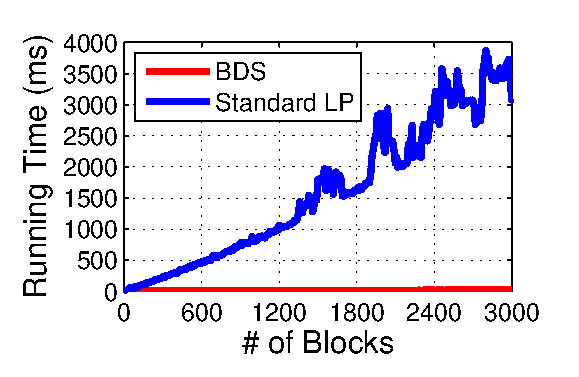
\includegraphics[width=50mm]{images/BDSvsLP.eps} % BDSvsLP.m
%                \caption{Algorithm running time of \name and standard LP.}
%                \label{fig:further:BDSvsLP}
%        \end{subfigure}
%        \begin{subfigure}[b]{0.3\textwidth}
%                \centering
%                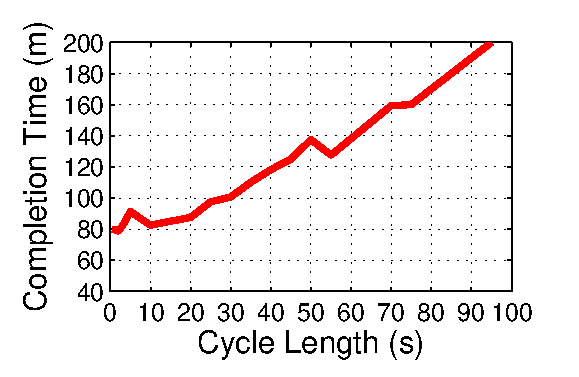
\includegraphics[width=50mm]{images/cycleDiff.eps}%cycleDiff.m
%                \caption{Completion time under different cycle lengths.}
%                \label{fig:further:cycleDiff}
%        \end{subfigure}
%        \begin{subfigure}[b]{0.3\textwidth}
%                \centering
%                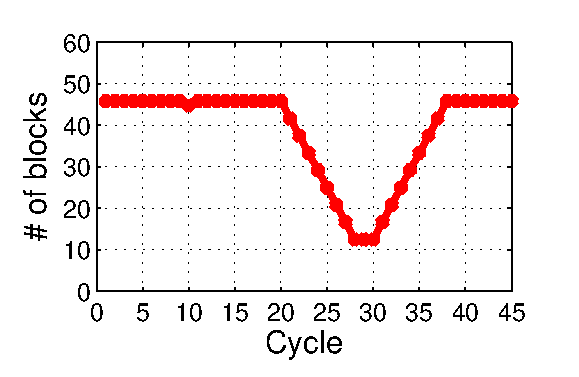
\includegraphics[width=50mm]{images/failure.eps}%fail.m
%                \caption{Average number of downloaded blocks per cycle under failures.}
%                \label{fig:further:failure}
%        \end{subfigure}
%        \caption{Further analysis on (1) running time, (2) cycle length, and (3) fault tolerance.}
%        \label{fig:further}
%\vspace{-0.4cm}
%\end{figure*}
\begin{figure*}[t]
        \centering
        \begin{subfigure}[b]{0.3\textwidth}
                \centering
                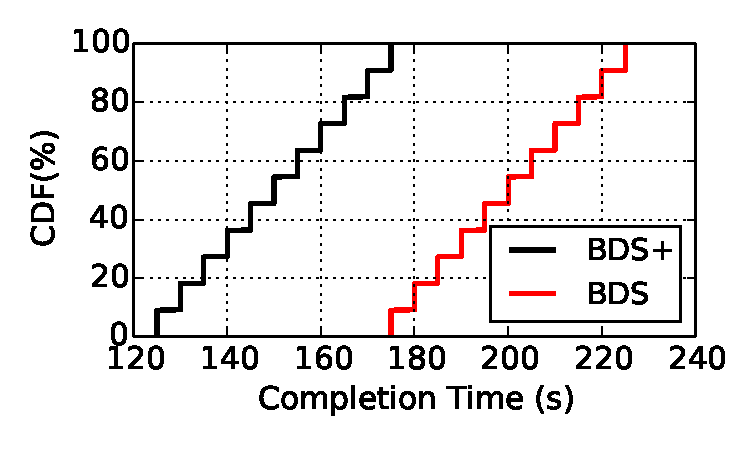
\includegraphics[width=50mm]{images/cdf_of_machine_completion_time.pdf}
                \caption{CDF of server completion time.}
                \label{fig:bdsplus:server}
        \end{subfigure}
        \begin{subfigure}[b]{0.3\textwidth}
                \centering
                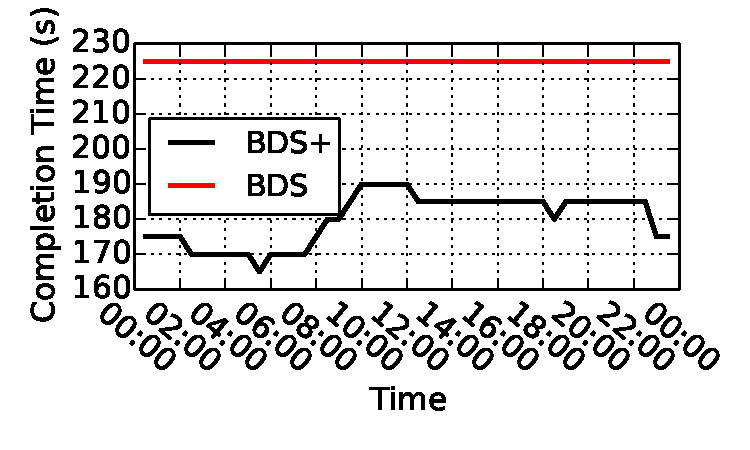
\includegraphics[width=50mm]{images/completion_time_period.pdf}
                \caption{Comparison at different periods.}
                \label{fig:bdsplus:periods}
        \end{subfigure}
        \begin{subfigure}[b]{0.3\textwidth}
                \centering
                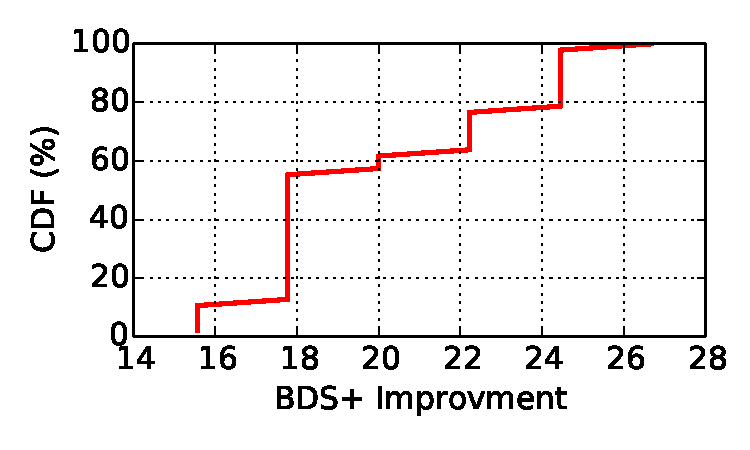
\includegraphics[width=50mm]{images/improvement_vs_bds.pdf}
                \caption{CDF of improvement.}
                \label{fig:bdsplus:vs}
        \end{subfigure}
        \tightcaption{[\newname vs. \name] Further improvements from \newname.}
        \label{fig:bdsplus}
%\vspace{-0.4cm}
\end{figure*}

\begin{figure*}[t]
        \centering
        \begin{subfigure}[b]{0.3\textwidth}
                \centering
                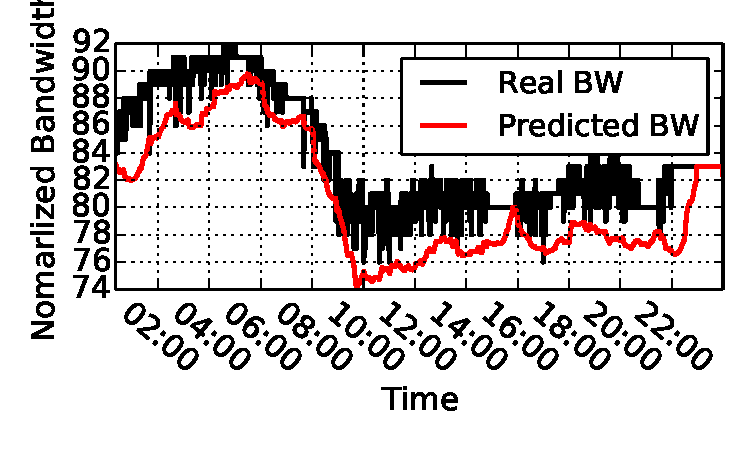
\includegraphics[width=50mm]{images/real_bw_and_estimate_bw.pdf}
                \caption{Available bandwidth and the predicted value.}
                \label{fig:pred:real}
        \end{subfigure}
        \begin{subfigure}[b]{0.3\textwidth}
                \centering
                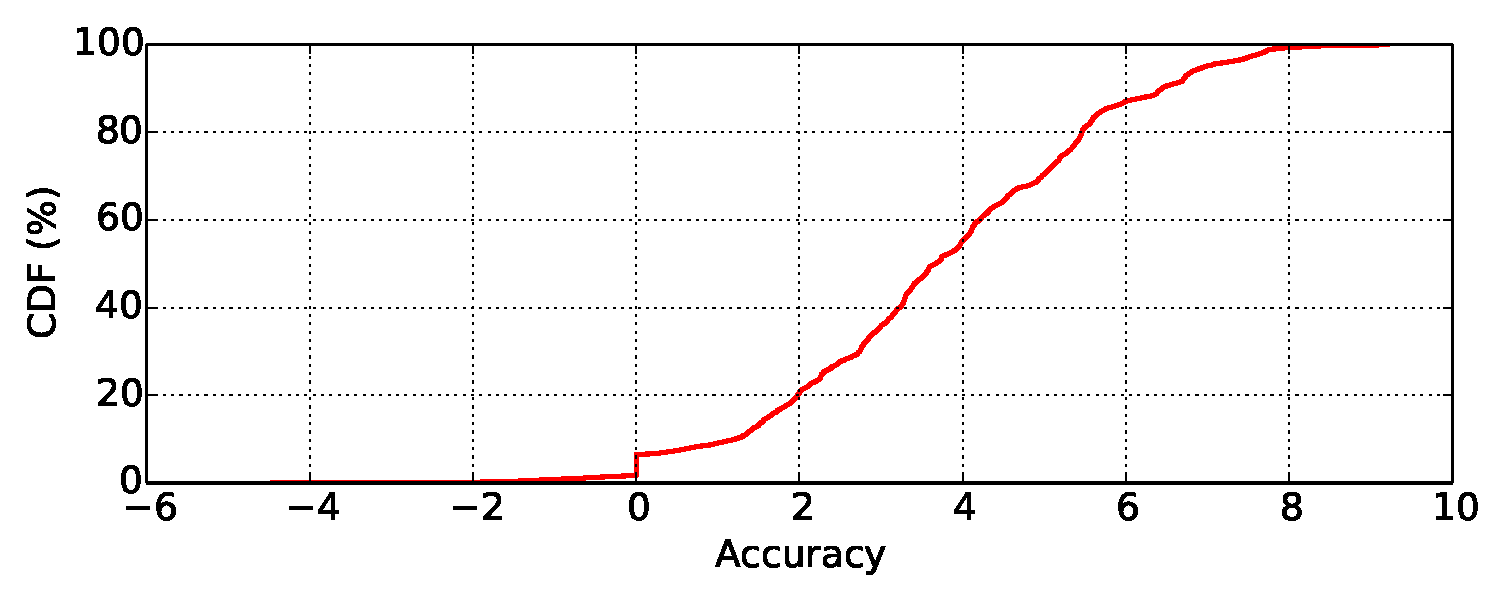
\includegraphics[width=50mm]{images/bw_prediction_accuracy.pdf}
                \caption{CDF of algorithm prediction accuracy.}
                \label{fig:pred:accurancy}
        \end{subfigure}
        \begin{subfigure}[b]{0.3\textwidth}
                \centering
                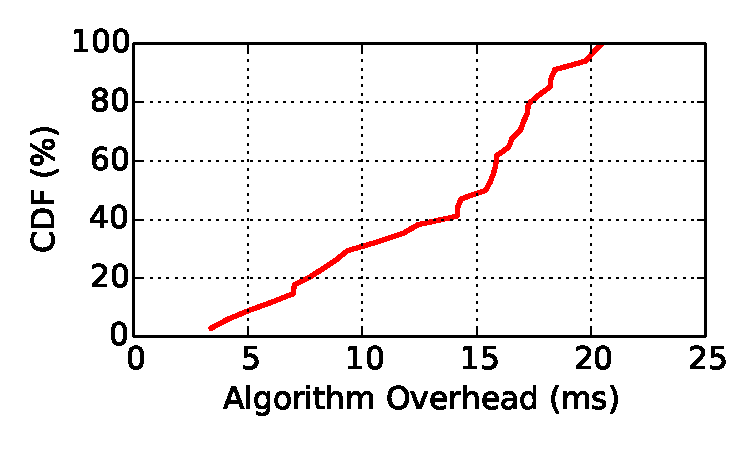
\includegraphics[width=50mm]{images/alg_overhead.pdf}
                \caption{Running time of the prediction algorithm.}
                \label{fig:pred:overhead}
        \end{subfigure}
        \tightcaption{[\newname's prediction algorithm] Evaluations on: (a) predicted value, (b) algorithm accuracy, (c) running time.}
        \label{fig:pred}
%\vspace{-0.4cm}
\end{figure*}

\NEW{
\subsection{\newname's dynamic bandwidth separation}
\label{subsec:evaluation:improvements}

\name reserves fixed size of bandwidth for online traffic (e.g., $20\%$), which is usually higher than the peak value. But lots of real traces show that online traffic rarely reaches the peak and is far below that in most cases. Thus, \newname adopts dynamic bandwidth seperation between online traffic and offline traffic, allowing offline traffic (bulk data transfer) to use more bandwidth when online traffic is below the threshold. \newname achieves this by an online traffic prediction algorithm, and this section shows the results of improved performance of \newname.

In the following experiments, we send 1TB data from one DC to 11 DCs, each has 100 servers, and the upload and download link capacities are set to be 20MBs. The online traffic is set according to the cluster trace (machine\_usage) from Ali \cite{datatrace}.

\subsubsection{Further improvements from \newname.}
\label{subsubsec:bdsplus:improvements}
\

\mypara{Completion time}
We start the bulk data transfer at 23:00 on 27, Jan, 2019. Figure~\ref{fig:bdsplus:server} shows the CDF of the completion time on each destination server. We can see that the average completion time of \newname is $150ms$, while that under \name takes more than $200ms$.

\mypara{Improvements over \name}
To make the results more general, we further conduct a series of experiments during different time periods, in other words, once per 30 minutes. We compare the completion time of both \newname and \name and show the results in Figure~\ref{fig:bdsplus:periods}. We can see that the improvements of \newname changes with time, specifically, the improvements during midnight is much higher than that during the day, especially at 05:30, when online traffic is at its valley. These results show that \newname can make full use of the idle bandwidth that is not used by online traffic. Overall, the CDF of improvements is shown in Figure~\ref{fig:bdsplus:vs}, which means that \newname can bring at least 18\% improvement in more than 85\% cases.

\subsubsection{\newname's prediction algorithm.}
\label{subsubsec:bdsplus:predict}
\

The improvement of \newname mainly comes from the prediction of online traffic, so in this subsection, we evaluate the accuracy of the prediction algorithm, and then analyze the overhead incurred in achieving such improvements.

\mypara{Algorithm accuracy} The online traffic is set according to the cluster trace (machine\_usage) from Ali \cite{datatrace}, the real residual bandwidth (the difference between server I/O and online traffic) is shown in black in Figure~\ref{fig:pred:real}, where the predicted value is shown in red. As we can see that the red line is smooth and quite close to the real bandwidth, indicating that \newname can predict online traffic precisely. The exact figures are shown in Figure~\ref{fig:pred:accurancy}, which indicates that the accuracy of about 99\% predictions is greater than 92\%. What's more, only in 1.6\% cases, \newname shows a little bit aggressiveness by gives a little bit higher predicted value (where the x-axis is below zero). In this way, \newname can not only increases bandwidth utilization when online traffic is in valley, but also reduces the incidents of interferences caused by bulk-data transfer.

\mypara{Algorithm overhead}
Although \newname bring performance improvements by making use of the residual bandwidth, it introduce some overhead on algorithm running time. So here we evaluate the additional time spent on making predictions on online traffic. Figure~\ref{fig:pred:overhead} shows the running time during a complete bulk data transfer. We can see that it takes less than $20ms$ for \newname to make predictions in more than 97\% cases. What's more, this overhead does not increase with system scale, because the prediction on each server is independent of each other and thus can be executed simultaneously.

In summary of all the above experiments, both the prototype pilot deployment and the trace-driven simulations of \name show 3-5$\times$ speedup over existing solutions, with good scalability and reliability, and near-optimal scheduling results. While the enhanced version \newname can work harmoniously with online traffic and further reduce the completion time of inter-DC multicasts, by making dynamic bandwidth separation.
}

%\begin{itemize}
%\item Scalability of centralized control:
%\begin{itemize}
%\item Y: Bandwidth consumption, vs. X: \# of objects
%\item Y: Controller CPU usage, vs. X: \# of objects
%\item Y: Update delay vs. X: \# of objects
%\item Bar-chart to decompose update delay into collecting updates, running algorithm, and updating local agents
%\end{itemize}
%
%\item In-depth analysis:
%\begin{itemize}
%\item A graph to show the tradeoff caused by different update cycles (why 3 seconds is a good tradeoff?)
%\item Reduction on algorithm running time due to the approximation algorithm.
%\item Maybe another graph from the current 6.3?
%\end{itemize}
%
%\item Fault tolerance:
%\begin{itemize}
%\item Y: flow completion time, vs. X: time. Create a toy topology to send objects. The experiment begins with no failure. At time t1, one server is not available, and the graph should show Y only has performance degradation for less than 3 seconds; At time t2, the controller is not available, and the local agent should automatically revert to decentralized local control.
%\end{itemize}
%
%\end{itemize}





